\documentclass[pra,12pt]{revtex4}
\usepackage{amsmath}
\usepackage{amssymb}
\usepackage{graphicx}
\usepackage{color}
\usepackage[pdfborder={0 0 0},colorlinks=true,linkcolor=blue]{hyperref}

\def\ket#1{\left|#1\right\rangle}
\def\bra#1{\left\langle#1\right|}
\def\braket#1{\left\langle#1\right\rangle}

\setlength{\parindent}{0pt}

\renewcommand{\baselinestretch}{1.0}
\setlength{\parskip}{0.07in}

\begin{document}

\section*{Appendix C: Entropy}

In classical contexts, ``entropy'' is a quantitative way to describe
our lack of knowledge about a system.  In information theory,
\textbf{information entropy} describes our uncertainty about the
contents of a message before receiving it.  In thermodynamics and
statistical mechanics, \textbf{thermodynamic entropy} describes our
uncertainty about the microscopic details (``microstate'') of a
complex many-body system.  In fact, these two formulations are
consistent with each other; for a description of how they are related,
see \hyperref[cite:feynman]{Feynman (2000)}.  Here, we will use the
statistical mechanics point of view.

Suppose a system has discrete microstates labeled by integers
$\{1,2,3,\dots\}$ , which have probabilities $\{p_1, p_2, p_3,
\dots\}$.  Then the entropy of the system is defined as
$$S_{\mathrm{cl.}} = - k_B \sum_{i} p_i \ln(p_i).$$
The probabilities $p_i$ are to be understood as \textit{conditional}
probabilities, conditioned on the known facts about the macroscopic
features of the system (e.g., we might know the total energy $E$).

If we know exactly which microstate the system is in (i.e., $p_k = 1$
for some state $k$), the entropy formula gives $S _{\mathrm{cl.}} =
0$.  The opposite situation, of ``complete uncertainty'', is provided
by a \textbf{micro-canonical ensemble}: a system that is at
equilibrium, has a fixed total energy $E$, and does not interact with
the rest of the universe.  In this case, the \textbf{ergodicity
  postulate} of statistical mechanics states that all possible
microstates with energy $E$ are equally probable.  If there are $W$
possible microstates, the probabilities are
$$p_i = \frac{1}{W} \;\;\forall i \in \{1,2,\dots,W\}.$$
Therefore, the entropy formula gives
$$S_{\mathrm{cl.}} \,=\, -k_B W \frac{1}{W} \ln(1/W) \;=\; k_B \ln W,$$
the famous result carved into the gravestone of Ludwig Boltzmann
(1844--1906).  Note that this expression has an implicit energy
dependence: changing $E$ varies $W$ and hence $S_{\mathrm{cl.}}$.

The entropy formula is designed so that any other probability
distribution, which describes a situation of \textit{partial}
uncertainty, yields an entropy $S_{\mathrm{cl.}}$ lying between $0$
and $k_B \ln W$.  To see that zero is the lower bound, first note that
for $0 \le p_i \le 1$, each term in the entropy formula satisfies
$-k_B\, p_i\ln(p_i) \ge 0$, and the equality holds if and only if $p_i
= 0$ or $p_i = 1$ (see the figure below):

\begin{figure}[h]
  \centering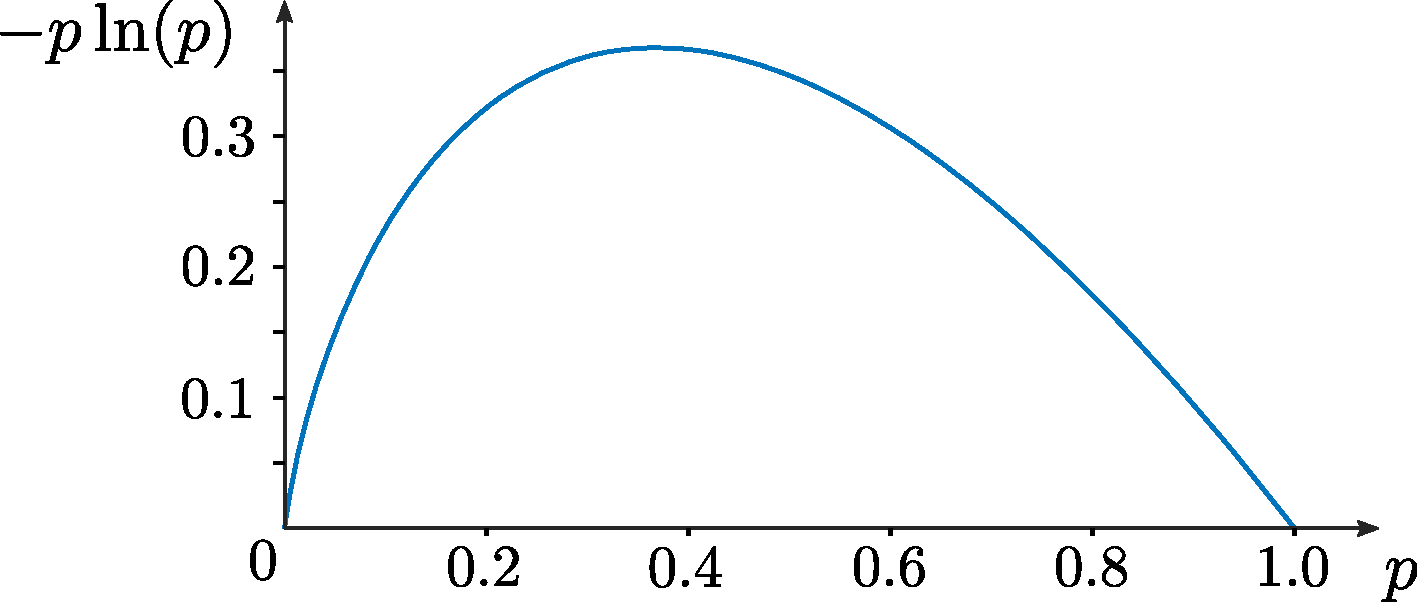
\includegraphics[width=0.7\textwidth]{plogp}
\end{figure}

This implies that $S_{\mathrm{cl.}}\ge 0$, and moreover that
$S_{\mathrm{cl.}} = 0$ if and only if $p_i = \delta_{ik}$ for some $k$
(i.e., there is no uncertainty).  Next, it can be shown that $k_B \ln
W$ is the upper bound (which implies the second law of
thermodynamics).  We will not go over the details of that proof, but
it follows from a mathematical relation known as
\href{https://en.wikipedia.org/wiki/Gibbs\%27_inequality}{Gibbs'
  inequality}.

Another important feature of the entropy formula is that
$S_{\mathrm{cl.}}$ is \textbf{extensive}, meaning that it scales
(``extends'') proportionally with system size.  To see this, consider
two independent systems A and B, which have microstate probabilities
$\{p_i^A\}$ and $\{p_j^B\}$.  If we regard the combination of A and B
as a single system, each microstate of the combined system is
specified by the microstate of A and the microstate of B, and is thus
indexed by integers $(i,j)$, with probability $p_{ij} = p^A_ip^B_j$.
The entropy of the combined system is
$$\begin{aligned}S_{\mathrm{cl.}} &= - k_B \sum_{ij} p_i^Ap^B_j \ln\left(p^A_ip^B_j\right) \\
  &= - k_B \Big(\sum_{i} p^A_i \ln p^A_i\Big)\Big(\sum_j p^B_j\Big)
  - k_B \Big(\sum_{i} p^A_i \Big) \Big(\sum_j p^B_j \ln p^B_j\Big) \\
  &= S_{\mathrm{cl.}}^A + S_{\mathrm{cl.}}^B,
\end{aligned}$$
where $S_{\mathrm{cl.}}^A$ and $S_{\mathrm{cl.}}^B$ are the individual
entropies of the A and B subsystems.

This has important consequences for the behavior of $W(E)$, the number
of microstates at each energy $E$.  Suppose we extend a system by
adding micro-canonical subsystems (which are insulated from each
other).  In the process, both $E$ and $S_{\mathrm{cl.}}$ increase
proportionally.  Since $S_{\mathrm{cl.}} \propto \ln[W(E)]$,
$$E \propto \ln W \;\;\;\Rightarrow \;\;\;W(E) \propto e^{\beta_0 E} \;\;\; \mathrm{for\;some}\; \beta_0 > 0.$$
If we relax the restriction that the additional subsystems are
micro-canonical, the number of microstates grows even faster with $E$,
as energy can now be distributed in different ways between the
subsystems.  It is reasonable to assume that the scaling is a
faster-growing exponential,
$$W(E) \propto e^{\beta E} \;\;\; \mathrm{for\;some}\; \beta \ge \beta_0.$$
This implies that the constant of proportionality relating
$S_{\mathrm{cl.}}$ and $E$ is
$$\frac{\partial E}{\partial S_{\mathrm{cl.}}} = \frac{1}{k_B \beta} = T,$$
where $\beta \equiv (k_BT)^{-1}$ \textit{defines} the temperature $T$.
This is the first law of thermodynamics.

A \textbf{canonical ensemble} is a system held in equilibrium with a
larger system, called a ``heat bath''.  We can model this with a
micro-canonical ensemble of energy $E$, divided into two subsystems, A
(the canonical ensemble) and B (the heat bath), which are not
insulated from each other.  Using the ergodicity postulate, and the
aforementioned exponential scaling of $W$ with $E$, one can show that
the probability for subsystem A to have energy $E_A$ is
$$p_A(E_A) \propto W_A(E_A) \, e^{-\beta E_A},$$
where $W_A(E_A)$ is the number of microstates of energy $E_A$ for
subsystem A, and $\beta$ is the inverse temperature of the heat bath.
This is the celebrated \textbf{Boltzmann law}.  It implies that each
microstate $i$, of energy $E_i$, has probability
$$p_i = \frac{\exp(-\beta E_i)}{Z}, \;\;\;\mathrm{where}\;\;Z \equiv \sum_j \exp(-\beta E_j).$$
$Z(\beta,E_1, E_2,\dots)$ is called the \textbf{partition function}.
Note that $p_i$ satisfies probability conservation, $\sum_i p_i = 1$,
and that the sum involves all microstates of all possible energies.

The probability distribution for a canonical ensemble represents a
partial-uncertainty situation, since lower-energy microstates are
more probable than higher-energy microstates.  Plugging the above
expression for $p_i$ into the entropy formula gives:
$$S_{\mathrm{cl.}} = \frac{1}{T} \frac{\sum_i E_i e^{-\beta E_i}}{\sum_i e^{-\beta E_i}} + k_B \ln Z \;=\; \frac{\langle E\rangle}{T} + k_B \ln Z,$$
where $\langle E\rangle = \sum_i E_i p_i$ denotes the average energy.
We can then define
$$F \,\equiv\, - k_B T \ln Z \,=\, \langle E \rangle - TS_{\mathrm{cl.}},$$
and show that this satisfies $\partial F/\partial T = -
S_{\mathrm{cl.}}$.  This quantity can be identified as the
thermodynamic \textbf{free energy}.

\end{document}
